\chapter{Referencial Teórico} \label{chap:referencial_teorico}

A pesquisa proposta nesta dissertação situa-se em um ponto de encontro entre duas tradições intelectuais que, por muito tempo, caminharam separadas. De um lado está a teoria financeira, preocupada em entender como os preços dos ativos se formam e como a informação se incorpora a eles. De outro está a Ciência da Computação, que oferece os instrumentos para representar e interpretar a linguagem humana em escala. Este capítulo costura essas duas tradições. Começa pela discussão teórica que justifica a própria possibilidade de extrair sinal preditivo de notícias, percorre o papel da mídia na formação de expectativas, examina a especificidade do ativo estudado, reconstrói a evolução das técnicas de Processamento de Linguagem Natural aplicadas a finanças, apresenta os fundamentos econométricos do risco e da fusão de dados e, ao final, sistematiza a literatura correlata por meio de uma revisão estruturada. A intenção é que, ao término da leitura, fique claro não apenas o que já foi feito, mas sobretudo onde se encontra a lacuna que este trabalho pretende preencher.

\section{A Hipótese de Mercados Eficientes}

O ponto de partida obrigatório de qualquer estudo sobre previsibilidade de preços é a Hipótese de Mercados Eficientes. Em sua formulação clássica, devida a \citeonline{fama_efficient_1970}, um mercado é eficiente quando os preços dos ativos refletem, a todo instante, a totalidade da informação disponível. A consequência dessa definição é severa para quem deseja prever retornos: se toda a informação já está no preço, então as variações futuras dependem apenas de informação ainda não revelada, que por definição é imprevisível. O preço passa a se comportar como um passeio aleatório, e a melhor estimativa para o valor de amanhã é o valor de hoje.

A teoria distingue três formas de eficiência, conforme a amplitude do conjunto informacional considerado. Na forma fraca, os preços incorporam apenas o histórico de cotações, de modo que a análise técnica baseada em padrões passados não geraria retornos anormais. Na forma semiforte, os preços refletem também toda a informação pública, o que inclui notícias, balanços e anúncios corporativos. Na forma forte, incorporam ainda a informação privada de agentes com acesso privilegiado. É a forma semiforte que interessa de maneira direta a esta dissertação, pois é nela que se coloca a questão central: o conteúdo de uma notícia financeira é absorvido pelos preços de modo instantâneo, ou resta, por algum intervalo mensurável, um resíduo de previsibilidade que um modelo computacional poderia explorar?

A hipótese, em sua versão mais rígida, não resistiu intacta ao escrutínio empírico. \citeonline{shiller_stock_1981} mostrou que os preços das ações oscilam muito mais do que seria justificável pelas variações nos dividendos futuros, sugerindo a presença de uma volatilidade em excesso incompatível com a racionalidade plena. Estudos posteriores documentaram anomalias persistentes. \citeonline{de_bondt_does_1985} encontraram evidência de que o mercado reage de forma exagerada a notícias, com reversões previsíveis no longo prazo, ao passo que \citeonline{jegadeesh_returns_1993} identificaram o efeito de momento, segundo o qual ativos que subiram tendem a continuar subindo por alguns meses. Diante desse acúmulo de evidências, mesmo defensores da hipótese passaram a admitir uma versão mais branda. \citeonline{malkiel_efficient_2003} reconhece que os mercados não são perfeitamente eficientes, mas argumenta que as ineficiências são pequenas, transitórias e difíceis de explorar depois de descontados os custos. É justamente nessa zona de quase-eficiência que esta pesquisa se posiciona: não se supõe a existência de um sinal forte e estável, e sim a possibilidade de um sinal fraco, porém real, capaz de deslocar a acurácia de um preditor alguns pontos percentuais acima do acaso.

Convém traduzir essas formas em termos operacionais para a tarefa preditiva desta dissertação. Sob a forma fraca, um preditor que use apenas o histórico de preços não deveria superar o acaso; sob a forma semiforte, tampouco um preditor que incorpore notícias públicas o faria de modo persistente. A previsão da direção diária de um ativo é, por isso, um teste exigente da própria hipótese: um desempenho sistematicamente acima de cinquenta por cento, ainda que por margem estreita, constitui evidência de ineficiência informacional explorável. É essa a régua adotada ao longo do trabalho, e por ela se deve julgar a magnitude, e não apenas o sinal, dos resultados. Cabe ressaltar, ademais, que mesmo um sinal estatisticamente real pode não ser economicamente explorável uma vez descontados os custos de transação. Essa distinção entre significância estatística e significância econômica, central à crítica de \citeonline{malkiel_efficient_2003} às anomalias, é honrada nesta dissertação ao se avaliar, além das métricas estatísticas, o desempenho de uma estratégia de negociação líquida de custos.

A defesa da eficiência não permaneceu inerte diante das anomalias. \citeonline{fama_market_1998} argumentou que muitas delas seriam fruto de metodologia ou de acaso, e que se distribuiriam de forma equilibrada entre reações exageradas e reações insuficientes, o que seria compatível com a eficiência. A controvérsia, longe de ser estéril, deslocou o debate para o conceito de limites à arbitragem. \citeonline{delong_noise_1990} demonstraram que a presença de investidores de ruído, que negociam com base em sentimento e não em fundamentos, pode afastar os preços do valor justo e, sobretudo, que o risco imposto por esses próprios investidores desencoraja os arbitradores racionais de corrigir o desvio. Disso resulta que as ineficiências podem persistir, e que o sentimento, longe de ser irrelevante, converte-se em um fator de risco com consequências sobre os preços. Essa perspectiva fornece o elo teórico entre a existência de um sinal de sentimento explorável e a sua natureza necessariamente limitada, coerente com a magnitude modesta dos efeitos que esta dissertação viria a documentar. Uma síntese acessível dessa transição, da teoria dos mercados eficientes para as finanças comportamentais, é oferecida por \citeonline{shiller_efficient_2003}.

\section{O Teorema da Concordância e o Papel da Informação}

Uma questão precede logicamente a discussão sobre o impacto das notícias: por que, afinal, a informação pública deveria mover os preços e gerar negociação? Uma resposta formal vem do teorema da concordância de \citeonline{aumann_agreeing_1976}, conhecido pela expressão concordar em discordar. Aumann demonstrou que, se dois agentes racionais partem de uma mesma probabilidade a priori e atualizam suas crenças pela regra de Bayes, e se as suas probabilidades a posteriori sobre um evento são de conhecimento comum, então essas probabilidades devem necessariamente coincidir. Em outras palavras, agentes plenamente racionais e com conhecimento comum não podem, de forma consistente, concordar em discordar sobre a probabilidade de um evento.

O teorema tem uma implicação importante para esta pesquisa. Se todos os investidores fossem perfeitamente racionais e compartilhassem o mesmo conjunto de informações, haveria pouca razão para negociar, pois as discordâncias tenderiam a se dissolver. O fato de existir intenso volume de negociação, e de os preços reagirem à chegada de notícias, indica que os investidores partem de crenças heterogêneas e processam a informação de maneiras distintas. A notícia pública funciona, nesse arcabouço, como o sinal que atualiza as probabilidades a posteriori dos agentes, e a forma como cada investidor interpreta o seu tom, otimista ou pessimista, ajuda a explicar a revisão das expectativas e o consequente movimento dos preços. Esse raciocínio foi levado ao limite por \citeonline{milgrom_information_1982}, cujo teorema da não-negociação demonstra que, partindo de crenças comuns e com racionalidade plena, a simples disposição de um agente a negociar revelaria informação privada e desencorajaria a contraparte, de modo que não haveria troca por motivo puramente especulativo. O enorme volume de negociação observado na prática é, portanto, um paradoxo sob a racionalidade estrita, e a sua explicação requer ou crenças heterogêneas, ou motivações de liquidez, ou desvios comportamentais. As notícias atuam exatamente sobre o primeiro desses canais, ao alimentar interpretações divergentes de um mesmo fato. O teorema da concordância e o seu corolário de não-negociação fornecem, assim, um fundamento racional para tratar o sentimento das notícias como informação economicamente relevante, que se soma à leitura comportamental apresentada na seção seguinte.

\section{Finanças Comportamentais}

Se a Hipótese de Mercados Eficientes fornece o pano de fundo, são as Finanças Comportamentais que fornecem o mecanismo pelo qual a informação textual poderia ter valor preditivo. Essa corrente parte de uma constatação simples e poderosa: os seres humanos não processam a informação como autômatos bayesianos perfeitos.

O marco fundador é a Teoria do Prospecto de \citeonline{kahneman_prospect_1979}, que demonstrou, por meio de experimentos, que as pessoas avaliam ganhos e perdas em relação a um ponto de referência, e não em termos de riqueza absoluta, e que sentem as perdas com intensidade maior do que os ganhos equivalentes. Esse fenômeno, conhecido como aversão à perda, tem uma implicação direta para o mercado: a reação a uma notícia ruim tende a ser mais aguda do que a reação a uma notícia boa de mesma magnitude. Em trabalho anterior, \citeonline{tversky_judgment_1974} já haviam catalogado um conjunto de heurísticas, como a representatividade, a disponibilidade e a ancoragem, que levam a desvios sistemáticos do julgamento sob incerteza.

A Teoria do Prospecto descreve esse comportamento por meio de uma função de valor com três propriedades que importam ao estudo das notícias. A função é definida sobre ganhos e perdas relativos a um ponto de referência, e não sobre a riqueza absoluta; é côncava no domínio dos ganhos e convexa no dos perdas, o que reflete a aversão ao risco diante de ganhos e a propensão ao risco diante de perdas; e é mais inclinada do lado das perdas, traduzindo numericamente a aversão à perda. A essa função soma-se uma ponderação não linear das probabilidades, que faz com que eventos raros, como grandes quedas, recebam peso desproporcional na decisão. Em conjunto, essas propriedades preveem que o investidor reagirá de modo assimétrico e mais intenso à informação negativa, fundamento microeconômico direto da hipótese de assimetria que esta dissertação testa empiricamente.

Os desvios não se limitam ao indivíduo isolado. No plano coletivo, o comportamento de manada leva os investidores a imitar as decisões alheias, amplificando movimentos iniciados por notícias e gerando bolhas e quedas abruptas. O efeito de disposição, por sua vez, descreve a tendência a vender cedo demais os ativos vencedores e a reter por tempo excessivo os perdedores, o que distorce a reação aos fundamentos. Tomados em conjunto, esses fenômenos sustentam a tese de que o fluxo de notícias, ao alimentar emoções e heurísticas, exerce sobre os preços um efeito que a racionalidade plena não preveria, efeito cuja intensidade e cujo sinal esta pesquisa procura quantificar.

Transposta para o agregado do mercado, a aversão à perda ajuda a explicar o chamado viés de negatividade, central para a terceira hipótese desta dissertação. Esse viés tem raízes cognitivas profundas: a psicologia documenta que eventos negativos exercem impacto maior do que eventos positivos de igual magnitude, princípio sintetizado na ideia de que o ruim é mais forte do que o bom \cite{baumeister_bad_2001, rozin_negativity_2001}. No plano da linguagem, isso se reflete em um vocabulário mais rico para descrever aspectos negativos, e os próprios léxicos de sentimento financeiro, como o de \citeonline{loughran_when_2011}, são compostos majoritariamente por termos negativos. Notícias de tom pessimista parecem provocar movimentos de preço e, sobretudo, picos de volatilidade mais intensos do que notícias otimistas. \citeonline{corredor_investor_2013} confirmaram essa assimetria em quatro mercados europeus e mostraram que a sua intensidade varia conforme características dos ativos e fatores culturais e institucionais de cada país, o que sugere que o efeito não é universal, mas dependente do contexto. No Brasil, \citeonline{silva_o_2018} ofereceu evidência convergente ao documentar que o sentimento das notícias afeta tanto o retorno quanto a volatilidade das ações.

O conceito de sentimento do investidor ganhou, com o tempo, estatuto próprio na literatura. \citeonline{baker_investor_2007} argumentaram que ondas de otimismo e pessimismo, difíceis de justificar por fundamentos, influenciam de modo sistemático os preços, em especial os de ações mais difíceis de arbitrar, como as de empresas pequenas, jovens ou voláteis. A PETR4, embora seja um papel de grande capitalização, compartilha um traço que a torna sensível a essas ondas: a sua forte exposição a fatores políticos, que alimentam narrativas e humores de mercado pouco ancorados em fundamentos estáveis.

\subsection{Modelos de reação e o papel da atenção}

A pesquisa comportamental não se limitou a catalogar vieses; propôs modelos formais que conciliam a evidência de reação exagerada no longo prazo com a de reação insuficiente no curto prazo. \citeonline{barberis_model_1998} construíram um modelo em que os investidores, ao alternarem entre regimes de crença, ora subreagem ora sobre-reagem às notícias, o que gera, respectivamente, momento de curto prazo e reversão de longo prazo. Em linha complementar, \citeonline{daniel_investor_1998} derivaram padrões semelhantes a partir do excesso de confiança e da atribuição enviesada, segundo os quais os investidores superestimam a precisão de sua informação privada. Esses modelos são relevantes para esta dissertação porque preveem que a reação do mercado ao conteúdo das notícias depende do horizonte e do estado de crença, o que motiva a análise do efeito do sentimento ao longo da distribuição do retorno, e não apenas na sua média.

Um segundo mecanismo, a atenção limitada, ajuda a explicar por que as notícias movem os preços mesmo quando não trazem fundamentos inteiramente novos. \citeonline{barber_all_2008} mostraram que ativos que ganham destaque na mídia atraem desproporcionalmente a atenção dos investidores individuais, gerando pressão de compra e movimentos de preço. A cobertura jornalística atua, portanto, não apenas como veículo de informação, mas como alocador de atenção, dimensão particularmente pertinente para um ativo de grande visibilidade midiática como a PETR4. Uma sistematização ampla desses mecanismos psicológicos e de seus efeitos sobre a precificação é apresentada por \citeonline{hirshleifer_investor_2001}. A Tabela~\ref{tab:vieses} resume os principais vieses e a sua implicação para o estudo do sentimento.

\begin{table}[htpb]
\centering
\caption{Principais vieses comportamentais e suas implicações para o efeito do sentimento das notícias.}
\label{tab:vieses}
\resizebox{0.98\textwidth}{!}{%
\begin{tabular}{p{3.2cm} p{5.4cm} p{5.6cm}}
\hline
\textbf{Viés} & \textbf{Descrição} & \textbf{Implicação para o sentimento} \\ \hline
Aversão à perda & As perdas pesam mais do que ganhos equivalentes & Reação assimétrica, mais intensa a notícias negativas \\
Excesso de confiança & Superestimação da precisão da própria informação & Sobre-reação às notícias, com reversão posterior \\
Atenção limitada & Capacidade restrita de processar a informação disponível & Notícias em destaque movem os preços por saliência \\
Ancoragem & Apego a valores de referência iniciais & Ajuste lento e incompleto às novas informações \\
Comportamento de manada & Imitação das decisões dos demais agentes & Amplificação dos efeitos do sentimento coletivo \\ \hline
\end{tabular}%
}
\vspace{0.2cm}
{\small \\ Fonte: Elaborado pelo autor com base na literatura citada.}
\end{table}

\section{A Mídia como Vetor de Informação}

Estabelecido que os investidores são sensíveis ao tom da informação, resta entender por qual canal essa informação chega até eles. A imprensa especializada é o canal por excelência, e a quantificação do seu efeito é o que aproxima as Finanças Comportamentais da computação.

O estudo seminal nessa direção é o de \citeonline{tetlock_giving_2007}, que construiu um índice de pessimismo a partir de uma coluna diária do \textit{Wall Street Journal} e mostrou que valores elevados de pessimismo antecedem quedas nos retornos do mercado, seguidas de uma reversão à média, além de se associarem a aumentos no volume negociado. O trabalho é importante por dois motivos. Primeiro, porque tratou o texto jornalístico como uma fonte de dados quantificável. Segundo, porque ofereceu uma interpretação econômica coerente com a teoria, na qual o pessimismo da mídia funciona como um indicador de sentimento que move temporariamente os preços para longe do seu valor fundamental.

A virada para as mídias sociais ampliou enormemente o volume de texto disponível. \citeonline{bollen_twitter_2011} mostraram que dimensões do humor coletivo extraídas de mensagens do Twitter antecipavam variações do índice Dow Jones, com ganho de acurácia na previsão direcional. \citeonline{antweiler_is_2004} já haviam investigado fóruns de discussão financeira e concluído que, embora boa parte do conteúdo seja ruído, há informação genuína capaz de prever volatilidade e volume. Na mesma linha, \citeonline{nguyen_sentiment_2015} incorporaram sentimentos associados a tópicos específicos extraídos de fóruns e obtiveram melhora sobre modelos baseados apenas em preços, reforçando a ideia de que o conteúdo temático, e não apenas a polaridade média, carrega sinal.

A natureza do efeito também foi esmiuçada em diferentes horizontes e fontes. \citeonline{li_effect_2014} analisaram o impacto conjunto de notícias corporativas e do humor público sobre os movimentos das ações e constataram que esse impacto varia conforme as características da empresa e o conteúdo da notícia. Em frequência ainda mais fina, \citeonline{gros-klusmann_when_2011} mediram intradiariamente a reação do mercado à leitura automatizada de notícias e mostraram que o ajuste de preços ocorre em minutos, o que torna a marcação temporal precisa um requisito incontornável para qualquer teste sério de causalidade. Esse achado antecipa, na literatura internacional, a exigência metodológica que se tornou o eixo da presente dissertação.

O efeito da mídia não é homogêneo entre países. \citeonline{calomiris_how_2019} analisaram um amplo painel internacional e concluíram que o fluxo de notícias e o seu contexto influenciam risco e retorno de forma estruturalmente mais severa em mercados emergentes do que em mercados desenvolvidos, o que se atribui à maior incerteza institucional e à menor profundidade desses mercados. Para o caso brasileiro, \citeonline{cardoso_whats_nodate} examinaram o impacto das manchetes sobre a atividade econômica nacional e evidenciaram a sensibilidade do ambiente de negócios ao noticiário, resultado que ampara a escolha do Brasil como objeto de estudo.

O acúmulo dessas evidências consolidou a análise textual como um campo próprio dentro das finanças, hoje sistematizado em revisões abrangentes \cite{kearney_textual_2014, loughran_textual_2016}. Desde os primeiros sistemas de extração de sentimento de fóruns na internet \cite{das_yahoo_2007}, a área amadureceu a ponto de separar o conteúdo informativo da notícia em si do sentimento que a acompanha. \citeonline{heston_news_2017}, por exemplo, mostraram que, mesmo controlando pela ocorrência da notícia, o seu tom ainda carrega poder preditivo sobre os retornos, o que reforça a pertinência de medir o sentimento de forma autônoma, tal como se faz nesta dissertação.

\section{A PETR4 e a Distinção entre Mercado e Ativo}

A escolha da PETR4 como objeto não é arbitrária, e a sua compreensão exige uma digressão sobre a economia do petróleo. As ações preferenciais da Petrobras reúnem, em um único papel, duas fontes de risco que nem sempre apontam na mesma direção.

A primeira fonte é o mercado internacional de petróleo. Como produtora da \textit{commodity}, a Petrobras tem suas receitas atadas ao preço do barril. A literatura econômica há muito investiga a relação entre o preço do petróleo e a economia. \citeonline{hamilton_oil_1983} documentou que quase todas as recessões norte-americanas do pós-guerra foram precedidas por elevações no preço do petróleo, estabelecendo o papel macroeconômico desses choques. Décadas depois, \citeonline{kilian_not_2009} refinou essa compreensão ao mostrar que nem todos os choques de preço do petróleo são iguais: é preciso distinguir choques de oferta, associados a interrupções de produção, de choques de demanda, ligados ao aquecimento da atividade global. Essa distinção tem uma consequência crucial para a presente pesquisa. Um evento geopolítico que reduza a oferta e eleve o preço do barril pode beneficiar a receita de uma produtora, ainda que represente uma má notícia para a economia como um todo e para o índice de ações. O mecanismo de transmissão é assimétrico conforme a origem do choque. Um choque de oferta, como o fechamento de uma rota de transporte ou um corte de produção, eleva o preço do petróleo e tende a aumentar a margem de uma produtora integrada, ao passo que um choque de demanda negativo, como uma recessão global que reduz o consumo, derruba simultaneamente o preço da \textit{commodity} e a atividade, prejudicando a empresa por duas vias. Para um índice amplo de ações, ambos os choques costumam ser desfavoráveis; para uma produtora de petróleo, porém, o primeiro pode ser favorável. É exatamente essa não trivialidade que torna inadequado tratar toda notícia de tom negativo sobre petróleo como sinal de queda para a PETR4, e que justifica o tratamento diferenciado por categoria temática adotado no método.

A segunda fonte de risco é política. Por ser uma empresa de capital misto, sob influência do Estado, a Petrobras tem suas decisões de preço, investimento e governança permeadas por considerações políticas. Isso a transforma em uma espécie de termômetro do risco institucional brasileiro, à semelhança do que \citeonline{baker_investor_2007} descrevem para ativos suscetíveis ao sentimento.

Da combinação dessas duas fontes emerge o ponto que a banca de qualificação levantou com precisão e que esta dissertação incorpora de forma explícita: uma notícia negativa para o mercado em geral não é necessariamente negativa para a PETR4 em particular. Uma guerra no Oriente Médio que derrube as bolsas mundiais pode, ao elevar o preço do petróleo, favorecer a produtora nacional. Tratar todo tom negativo como sinal de queda do ativo seria, portanto, um erro de interpretação econômica. A solução adotada no método, descrita no Capítulo~\ref{chap:metodologia}, é a organização das notícias por uma taxonomia temática que separa eventos da empresa de eventos do mercado de petróleo, permitindo que o sentido econômico de cada categoria seja considerado.

\section{Incerteza Econômica como Condicionante}

A literatura sugere que o efeito das notícias sobre os preços não é constante, e sim mais intenso em períodos de turbulência. Para tratar essa heterogeneidade de forma rigorosa, é necessário precisar o conceito de incerteza econômica. A distinção seminal é a de \citeonline{knight_risk_1921}, que separou risco de incerteza: o risco refere-se a situações em que a distribuição de probabilidade dos resultados é conhecida, ao passo que a incerteza, em sentido estrito, descreve situações em que essa distribuição é desconhecida. \citeonline{bloom_fluctuations_2014} associa a incerteza às dúvidas dos agentes sobre o futuro, relacionando-a a fenômenos macroeconômicos e microeconômicos, enquanto \citeonline{jurado_measuring_2015} a operacionalizam como a volatilidade condicional da parcela imprevisível das expectativas.

Como a incerteza não é diretamente observável, a literatura recorre a aproximações. Uma das mais influentes é o índice de incerteza de política econômica de \citeonline{baker_measuring_2016}, construído, de forma sugestiva para esta pesquisa, a partir da frequência de termos relacionados à incerteza em jornais, o que evidencia que o próprio texto noticioso carrega informação sobre o estado de incerteza da economia. A relevância desse conceito para a presente dissertação é dupla. Primeiro, porque a evidência de que o sentimento das notícias afeta mais os preços em períodos de recessão \cite{garcia_sentiment_2013} sugere que o seu poder preditivo deve ser avaliado de modo sensível ao regime de mercado. Segundo, porque a própria volatilidade condicional estimada pelo GARCH funciona como uma aproximação do nível de incerteza do mercado, o que liga diretamente a modelagem de risco à análise do sentimento. Essa articulação motiva as análises por subperíodo e por regime conduzidas no Capítulo~\ref{chap:resultados}.

\section{Processamento de Linguagem Natural em Finanças}

A capacidade de transformar texto em sinal numérico é o que viabiliza tudo o que foi discutido até aqui. Esta seção reconstrói a evolução dessa capacidade em quatro estágios sucessivos, cada um superando limitações do anterior.

\subsection{A distribuição das palavras: a Lei de Zipf}

Antes de representar um texto numericamente, é útil compreender uma regularidade estatística da linguagem que condiciona todas as técnicas de mineração textual. Ao estudar a frequência das palavras em obras literárias, \citeonline{zipf_human_1949} observou que a frequência de uma palavra é aproximadamente inversamente proporcional à sua posição em um \textit{ranking} de ocorrências, de modo que o produto entre a frequência e a posição permanece quase constante. Essa regularidade, conhecida como lei de Zipf, implica que poucas palavras são extremamente frequentes, enquanto a imensa maioria do vocabulário ocorre muito raramente. Para as palavras de baixa frequência, \citeonline{booth_law_1967} formulou uma lei complementar.

A lei de Zipf tem consequências diretas para a análise de sentimento. De um lado, as palavras mais frequentes tendem a ser conectivos e termos genéricos, de baixo poder discriminante, o que justifica a sua remoção ou o seu rebaixamento por esquemas de ponderação como o TF-IDF. De outro, o conteúdo informativo concentra-se em termos relativamente raros e específicos do domínio, o que explica por que as representações baseadas apenas em contagem enfrentam o problema da esparsidade, e por que modelos contextuais, capazes de inferir o significado de uma palavra a partir de poucas ocorrências e do seu entorno, representam um avanço. Essa compreensão fundamenta tanto a construção da taxonomia de termos adotada no método quanto a opção por um modelo de linguagem contextual.

A Figura~\ref{fig:zipf} confirma a validade da lei de Zipf no corpus desta pesquisa. Ao ordenar as palavras das notícias da PETR4 pela frequência e plotar a frequência contra a posição em escala logarítmica, obtém-se uma reta descendente próxima da curva teórica, o que evidencia que pouquíssimas palavras concentram a maior parte das ocorrências, enquanto a vasta maioria do vocabulário, de mais de quarenta mil palavras distintas, aparece raramente.

\begin{figure}[htpb]
\centering
\caption{Distribuição de frequência das palavras no corpus de notícias da PETR4, em escala logarítmica, comparada à curva teórica da lei de Zipf. A aderência confirma a concentração das ocorrências em poucos termos.}
\vspace{0.2cm}
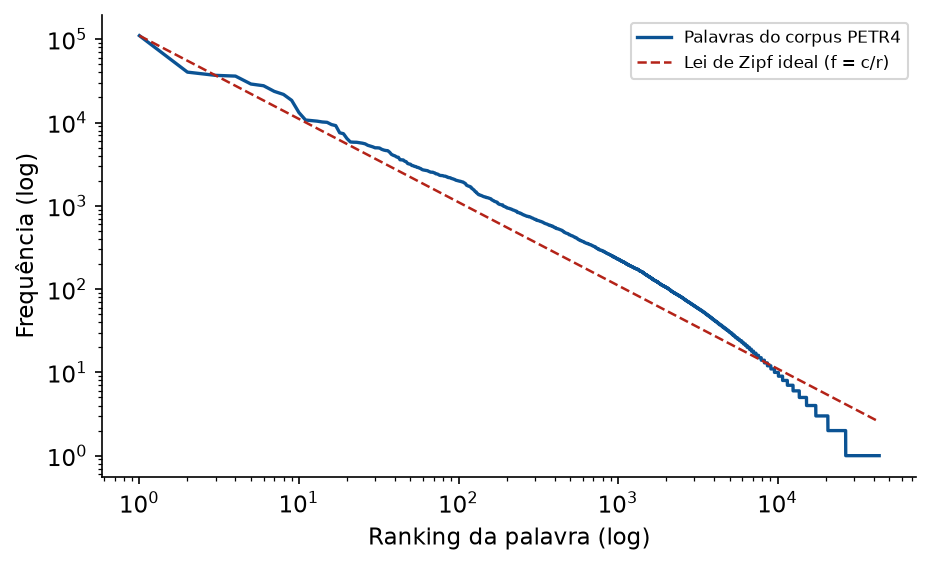
\includegraphics[width=0.75\textwidth]{figuras/fig_zipf.png}
\label{fig:zipf}
\vspace{0.2cm}
{\small Fonte: Elaborado pelo autor.}
\end{figure}

\subsection{Representações léxicas e de contagem}

As primeiras aplicações representavam um documento como um vetor de frequências de palavras, abordagem conhecida como \textit{Bag-of-Words}. A variante mais difundida, o TF-IDF, pondera cada termo pela sua frequência no documento e pela sua raridade no conjunto, de modo a destacar palavras discriminantes. No mercado brasileiro, \citeonline{nizer_metodo_2011} foi precursor ao empregar essa família de técnicas para detectar o efeito de publicações de notícias sobre ações da Bovespa, em um trabalho que abriu caminho para a pesquisa nacional na área.

Para tornar a contagem sensível ao domínio, desenvolveram-se léxicos de sentimento, isto é, listas de palavras previamente classificadas como positivas ou negativas. A contribuição decisiva nessa linha foi a de \citeonline{loughran_when_2011}, que demonstraram que dicionários de uso geral classificam de forma equivocada o vocabulário financeiro: termos como passivo, custo ou imposto, neutros ou meramente técnicos em finanças, seriam contados como negativos por um léxico genérico. A construção de um dicionário financeiro específico, hoje referência consolidada na área, corrigiu esse viés e melhorou substancialmente a medição do tom. Ainda assim, todos os métodos dessa família partilham a limitação estrutural já apontada: ao representar o texto como um conjunto de palavras independentes, ignoram a negação, a ironia e a dependência de contexto, de modo que as frases resultado acima do esperado e resultado abaixo do esperado, que diferem em uma única palavra mas têm sentidos opostos, podem receber tratamento semelhante. A superação dessa limitação foi o motor da evolução descrita nas subseções seguintes.

O reconhecimento de que o vocabulário financeiro tem conotações próprias levou ao desenvolvimento de léxicos especializados. \citeonline{loughran_when_2011} demonstraram que listas de palavras negativas de uso geral classificam erroneamente muitos termos no contexto financeiro, pois palavras como passivo ou imposto não carregam, nesse domínio, a carga negativa que teriam em outro. A criação de um dicionário financeiro específico melhorou de forma sensível a análise. Ainda assim, todas essas representações compartilham uma limitação de fundo: ao tratar o texto como um saco de palavras, descartam a ordem e a sintaxe, o que as torna incapazes de interpretar negações, ironias e construções dependentes do contexto, frequentes no jornalismo de mercado.

\subsection{Aprendizado de máquina e seleção de atributos}

O estágio seguinte associou as representações textuais a classificadores de aprendizado de máquina, capazes de aprender fronteiras de decisão a partir de exemplos. \citeonline{schumaker_quantitative_2009} construíram o sistema AZFinText, que combinou informação de preços a atributos textuais por meio de máquinas de vetores de suporte e foi um dos primeiros sistemas quantitativos de previsão baseados em notícias a apresentar resultados de negociação simulada. \citeonline{hagenau_automated_2013} avançaram ao mostrar que atributos sensíveis ao contexto das sentenças, e não apenas a contagem isolada de palavras, elevam a acurácia da previsão.

À medida que o número de atributos textuais cresce, surge o problema da alta dimensionalidade, que prejudica o desempenho dos classificadores. \citeonline{odhiambo_omuya_feature_2021} enfrentaram esse problema com técnicas de seleção de atributos baseadas em ganho de informação, obtendo modelos mais enxutos e precisos. No tocante à escolha do algoritmo, \citeonline{ballings_evaluating_2015} conduziram uma avaliação extensa de múltiplos classificadores para a previsão direcional binária e apontaram métodos baseados em árvores e em margens, como o \textit{Random Forest} e as máquinas de vetores de suporte, entre os mais adequados, conclusão que ampara a escolha dos classificadores empregados nesta dissertação. Arquiteturas híbridas, que combinam componentes lineares e não lineares, também se mostraram úteis, como demonstrou \citeonline{wang_stock_2012} ao mesclar modelos de séries temporais a redes neurais para a previsão de índices. O problema da alta dimensionalidade, conhecido como maldição da dimensionalidade, é particularmente agudo na análise textual, pois o vocabulário de um corpus pode conter dezenas de milhares de termos, cada um dando origem a um atributo. Nesse regime, o número de atributos rivaliza ou supera o número de observações, o que facilita o sobreajuste e degrada a generalização. As respostas a esse problema seguem duas direções complementares: a seleção de atributos, que descarta os termos pouco informativos, e a redução de dimensionalidade, que projeta os atributos em um espaço menor. A taxonomia temática adotada nesta dissertação pode ser entendida como uma forma supervisionada e interpretável de redução de dimensionalidade, na qual milhares de termos possíveis são condensados em sete dimensões de sentimento, uma por categoria, sem a perda de interpretabilidade que acompanharia uma projeção puramente estatística.

\subsection{Representações distribuídas de palavras}

Um avanço intermediário entre a contagem de palavras e os modelos contextuais foi a introdução das representações distribuídas, conhecidas como \textit{word embeddings}. Em vez de tratar cada palavra como um símbolo isolado, esses métodos a representam por um vetor denso, aprendido de modo que palavras de significado semelhante ocupem posições próximas no espaço vetorial. O modelo \textit{word2vec}, de \citeonline{mikolov_efficient_2013}, e o \textit{GloVe}, de \citeonline{pennington_glove_2014}, popularizaram essa ideia ao aprender vetores a partir de grandes corpora, capturando relações semânticas e sintáticas que a representação \textit{Bag-of-Words} ignora. Os \textit{embeddings} atenuaram o problema da esparsidade apontado pela lei de Zipf, mas ainda atribuíam a cada palavra um único vetor, independentemente do contexto, limitação que só seria plenamente superada pelos modelos contextuais discutidos a seguir.

\subsection{Aprendizado profundo}

A terceira virada veio com o aprendizado profundo, que dispensou a engenharia manual de atributos ao aprender representações diretamente dos dados. As redes neurais convolucionais, originalmente concebidas para imagens, foram adaptadas ao texto ao deslizar filtros sobre sequências de palavras, detectando padrões locais como expressões e combinações de termos relevantes, independentemente da posição em que ocorrem na frase. As redes recorrentes, por sua vez, processam a sequência elemento a elemento e mantêm um estado interno que resume o que foi lido, modelando a dependência entre as palavras. \citeonline{vargas_deep_2017} aplicaram essa combinação a artigos de notícias financeiras e mostraram que a memória sequencial das redes recorrentes captura relações que as abordagens de contagem ignoram. A Figura~\ref{fig:vargas} reproduz a arquitetura proposta por esses autores, na qual a camada convolucional extrai características semânticas locais e a camada recorrente preserva o contexto sequencial das notícias.

\begin{figure}[htpb]
\centering
\caption{Arquitetura de aprendizado profundo que combina uma camada convolucional, responsável por características locais, e uma camada recorrente, responsável pela memória sequencial das notícias, aplicada à previsão do mercado financeiro a partir de texto.}
\vspace{0.2cm}
\includegraphics[width=0.8\textwidth]{figuras/arquitetura_nlp_vargas.png}
\label{fig:vargas}
\vspace{0.2cm}
{\small Fonte: Adaptado de \citeonline{vargas_deep_2017}.}
\end{figure}

Apesar do avanço, as redes recorrentes sofrem de uma limitação prática conhecida como o problema do gradiente que se desvanece: ao processar as frases palavra por palavra e propagar o erro por muitas etapas, a influência dos termos iniciais sobre os finais tende a se dissipar, o que dificulta a retenção de dependências entre termos distantes. A arquitetura de memória de longo e curto prazo, proposta por \citeonline{hochreiter_long_1997}, atenuou esse problema ao introduzir portões que regulam o fluxo de informação ao longo da sequência, e por isso dominou o processamento de texto durante anos. Ainda assim, a leitura estritamente sequencial impunha um teto à capacidade de relacionar termos muito afastados e impedia a paralelização eficiente do treinamento. Foi a superação dessas duas limitações que abriu o estágio seguinte.

\subsection{Transformers, BERT e modelos de domínio}

A arquitetura \textit{Transformer}, introduzida por \citeonline{vaswani_attention_2017}, eliminou a leitura sequencial. Em seu lugar, o Mecanismo de Atenção processa todos os termos de uma sentença de forma simultânea e calcula, para cada par de palavras, um peso que mede o quanto uma deve influenciar a representação da outra. Esse mecanismo permite que o modelo capte, em uma única operação, relações de longo alcance que as redes recorrentes só alcançavam com dificuldade.

Sobre esse alicerce, \citeonline{devlin_bert_2019} propuseram o BERT, sigla de \textit{Bidirectional Encoder Representations from Transformers}. O modelo é pré-treinado em grandes volumes de texto por meio de tarefas auto-supervisionadas, como prever palavras mascaradas, e aprende representações contextuais profundas que podem ser reaproveitadas em tarefas específicas. Esse desenho consagra o paradigma da transferência de aprendizado, no qual o conhecimento linguístico geral, adquirido a alto custo computacional sobre um corpus massivo, é transferido para uma tarefa particular mediante um ajuste fino relativamente barato, com poucos exemplos rotulados. A vantagem é dupla: dispensa-se o treinamento de um modelo do zero para cada nova tarefa, e aproveita-se a competência linguística geral mesmo quando os dados rotulados da tarefa-alvo são escassos, situação típica da análise de sentimento financeiro em português. É importante, neste ponto, fixar uma distinção conceitual que a banca destacou e que será retomada no método: o BERT é um codificador. Ele transforma o texto em vetores numéricos, mas não produz, por si só, um rótulo de sentimento. Para classificar, é preciso acoplar ao codificador um cabeçalho de classificação e ajustá-lo com exemplos rotulados da tarefa de interesse.

Para o português brasileiro, \citeonline{souza_bertimbau_2020} treinaram o BERTimbau, um BERT nativo da língua, que se tornou referência para tarefas de PLN em português. \citeonline{narde_classificacao_nodate} validaram a aplicação de modelos dessa família à classificação de notícias no idioma, atestando o seu desempenho. Resta, contudo, um problema de domínio. Um modelo treinado em texto de propósito geral, ainda que no idioma correto, não garante a compreensão do vocabulário e do sentido econômico do noticiário financeiro, simplesmente porque esse domínio é pouco representado em seus dados de treinamento. Afirmar que um modelo genérico desambígua, por si, jargões e ironias do mercado seria uma sobre-estimação, como bem apontou a banca de qualificação.

A resposta a esse problema é o ajuste fino de domínio. A estratégia foi consagrada, para o inglês, pelo FinBERT de \citeonline{araci_finbert_2019}, que adaptou o BERT a textos financeiros e superou os modelos genéricos na classificação de sentimento do setor. O FinBERT-PT-BR, proposto por \citeonline{santos_finbert_2023}, transpõe essa ideia para o português e é, precisamente, o BERTimbau especializado em finanças. Os autores conduziram um pré-treinamento adicional sobre mais de um milhão de textos financeiros em português e, a partir dele, ajustaram um classificador de sentimento de três classes com um conjunto rotulado, reportando desempenho superior a linhas de base do estado da arte. A adoção desse modelo nesta dissertação se justifica por reunir, em um só artefato, a competência linguística do BERTimbau e a especialização no domínio, o que dispensa a construção, a partir do zero, de um amplo corpus financeiro anotado. Em outras palavras, optar pelo FinBERT-PT-BR em vez do BERTimbau genérico não significa trocar de família de modelo, e sim empregar o mesmo modelo já adaptado à tarefa e ao domínio exatos da pesquisa.

\section{Fundamentos dos Algoritmos de Classificação}

A previsão de direção apoia-se em algoritmos cuja mecânica convém apresentar, pois a sua escolha não é acidental e responde a propriedades específicas do problema. Esta seção expõe os fundamentos do mecanismo de atenção, que sustenta a extração de sentimento, e dos dois classificadores empregados na decisão direcional.

\subsection{O mecanismo de atenção}

As redes recorrentes, e em particular a variante de memória de longo e curto prazo proposta por \citeonline{hochreiter_long_1997}, foram durante anos a ferramenta padrão para processar sequências, pois introduziram uma memória capaz de reter informação ao longo do tempo. Elas processam o texto de forma sequencial, um termo após o outro, o que limita a sua capacidade de relacionar palavras muito distantes e dificulta a paralelização do treinamento. O mecanismo de atenção, introduzido por \citeonline{vaswani_attention_2017}, supera essas limitações. A sua ideia central é calcular, para cada par de termos de uma sentença, um peso que mede o quanto um termo deve influenciar a representação do outro. Cada termo gera três vetores, denominados consulta, chave e valor, e a compatibilidade entre a consulta de um termo e a chave de outro determina o peso atribuído ao valor correspondente. Uma analogia útil é a de um sistema de busca: a consulta de uma palavra é confrontada com as chaves de todas as demais, e as palavras cujas chaves melhor correspondem à consulta têm seus valores recuperados com maior peso na nova representação. Assim, ao processar a palavra alta em uma manchete, o mecanismo pode atribuir grande peso a uma palavra próxima como queda ou greve, ajustando o seu significado ao contexto. Como esse cálculo é feito simultaneamente para todos os pares, o modelo capta relações de longo alcance em uma única operação e permite o treinamento paralelo em grande escala, vantagem que viabilizou o treinamento de modelos de linguagem em corpora massivos. É esse mecanismo que confere ao BERT \cite{devlin_bert_2019} e, por extensão, ao FinBERT-PT-BR a capacidade de interpretar o contexto de uma manchete financeira de forma sensível à ordem e à coocorrência das palavras.

\subsection{Máquinas de vetores de suporte}

A máquina de vetores de suporte, formalizada por \citeonline{cortes_support_1995}, é um classificador que busca o hiperplano de separação entre duas classes que maximiza a margem, isto é, a distância até os exemplos mais próximos de cada classe. Esses exemplos críticos, chamados vetores de suporte, definem sozinhos a fronteira de decisão, o que confere robustez ao método. Quando as classes não são linearmente separáveis, recorre-se ao chamado truque do núcleo, que projeta os dados em um espaço de dimensão mais alta no qual a separação linear se torna possível, sem que essa projeção precise ser calculada de forma explícita. O núcleo de base radial, empregado nesta dissertação, é adequado a fronteiras não lineares em espaços de baixa dimensão, situação compatível com o pequeno número de atributos da matriz de fusão. A maximização da margem tem uma justificativa teórica profunda: fronteiras de margem ampla tendem a generalizar melhor para dados não vistos, princípio ligado à teoria do aprendizado estatístico. Na prática, como as classes raramente são perfeitamente separáveis, emprega-se a chamada margem suave, que admite alguns erros de classificação mediante uma penalidade, controlada por um hiperparâmetro de regularização que equilibra a largura da margem e a tolerância a erros. Esse equilíbrio é especialmente delicado em dados financeiros, nos quais um modelo excessivamente ajustado captura ruído em vez de sinal. A escolha da máquina de vetores de suporte como um dos classificadores é amparada pela avaliação de \citeonline{ballings_evaluating_2015}, que a apontou entre os métodos mais adequados à previsão direcional. Cabe observar, ainda, que a máquina de vetores de suporte é sensível à escala dos atributos, razão pela qual a sua aplicação é precedida de uma padronização, ajustada estritamente sobre os dados de treino para evitar o vazamento de informação.

\subsection{Gradient boosting e XGBoost}

A segunda família de classificadores é a do \textit{gradient boosting}, formalizada por \citeonline{friedman_greedy_2001}. A sua estratégia consiste em construir, de forma aditiva e sequencial, um conjunto de modelos simples, em geral árvores de decisão rasas, em que cada novo modelo é treinado para corrigir os erros residuais dos anteriores. O resultado é um preditor forte, obtido pela soma ponderada de muitos preditores fracos, que aprende relações não lineares e interações entre atributos sem que estas precisem ser especificadas a priori. O \textit{Extreme Gradient Boosting}, ou XGBoost, proposto por \citeonline{chen_xgboost_2016}, é uma implementação escalável dessa ideia, que incorpora termos de regularização para controlar a complexidade do modelo e mitigar o sobreajuste, além de técnicas de paralelização e de tratamento eficiente de valores ausentes. Duas características do XGBoost são especialmente úteis a esta pesquisa. A primeira é a sua robustez como método de referência para dados tabulares, confirmada por \citeonline{nobre_combining_2019} no domínio financeiro. A segunda é a possibilidade de extrair a importância de cada atributo, medida pela contribuição às divisões das árvores, que viabiliza a análise de ablação conduzida no Capítulo~\ref{chap:resultados}.

A escolha do XGBoost para a tarefa direcional não é casual, e reflete propriedades particularmente adequadas ao problema. Em primeiro lugar, os dados financeiros aqui empregados são tabulares e de baixa dimensão, regime em que os métodos baseados em árvores costumam superar as redes neurais profundas, mais adequadas a dados de alta dimensão como imagens e texto bruto. Em segundo lugar, a regularização explícita do XGBoost é uma defesa importante contra o sobreajuste, risco elevado quando o sinal é fraco e o ruído é alto, exatamente o cenário de um mercado quase-eficiente. Em terceiro lugar, a sua capacidade de modelar interações entre atributos permite captar relações como a de que o sentimento importa mais sob alta volatilidade, que um modelo linear não representaria sem termos de interação explícitos. Essas vantagens, somadas à interpretabilidade pela importância de atributos, fazem do XGBoost a escolha natural para o núcleo preditivo desta dissertação, ainda que o estudo de refinamento venha a mostrar que, neste problema específico, a sua versão mais parcimoniosa é a mais robusta.

\subsection{Avaliação em séries temporais financeiras}

A avaliação de modelos preditivos em finanças é tão importante quanto a sua construção, e está sujeita a armadilhas específicas que convém explicitar. A mais grave é o vazamento de informação, que ocorre quando o procedimento de avaliação permite ao modelo acessar, ainda que de forma indireta, dados do futuro. A validação cruzada tradicional, que embaralha as observações, é inadequada às séries temporais por essa razão, pois rompe a ordem cronológica e contamina o treino com informação posterior. A alternativa consagrada é a validação cronológica, conhecida como \textit{walk-forward}, em que o modelo é sempre treinado sobre um passado e avaliado sobre um futuro, simulando o uso real \cite{henrique_literature_2019}. Uma segunda dificuldade é o problema da hipótese conjunta: ao testar a previsibilidade, testa-se simultaneamente o modelo de previsão e a própria hipótese de eficiência, de modo que um resultado negativo não distingue entre um modelo inadequado e um mercado eficiente. Por fim, a comparação entre modelos exige cuidado estatístico, e instrumentos como o teste de \citeonline{diebold_comparing_1995} permitem aferir se a diferença de acurácia entre dois preditores é significativa, e não fruto do acaso. Esta dissertação incorpora essas três precauções: adota a divisão estritamente cronológica, interpreta os resultados à luz da quase-eficiência e reporta testes formais de significância.

\section{Econometria do Risco}

A dimensão de risco da pesquisa, ligada à volatilidade, exige um tratamento econométrico próprio. As séries de retornos financeiros raramente apresentam variância constante ao longo do tempo. Em vez disso, exibem o fenômeno do agrupamento de volatilidade, observado já por analistas clássicos e formalizado na econometria moderna: períodos de grandes oscilações tendem a ser seguidos por novas grandes oscilações, e períodos de calmaria por nova calmaria.

O reconhecimento de que a variância dos retornos não é constante, mas varia no tempo de modo previsível, representou uma virada na econometria financeira, premiada posteriormente com o Nobel. A modelagem desse comportamento começou com o modelo ARCH de \citeonline{engle_autoregressive_1982}, que expressou a variância de um período como função dos quadrados dos erros passados, capturando assim a ideia de que choques recentes elevam a incerteza corrente. A intuição é direta: um dia de forte oscilação aumenta a expectativa de oscilação no dia seguinte, o que reproduz matematicamente o agrupamento de volatilidade observado nos dados. A generalização proposta por \citeonline{bollerslev_generalized_1986}, o modelo GARCH, acrescentou a essa estrutura a dependência da própria variância passada, o que permitiu descrever a persistência da volatilidade com poucos parâmetros. A especificação GARCH(1,1), com uma defasagem de cada termo, tornou-se o cavalo de batalha da econometria financeira por reunir parcimônia e bom ajuste empírico, e a soma dos seus dois coeficientes fornece uma medida direta da persistência da volatilidade. Para acomodar as caudas pesadas características dos retornos, isto é, a ocorrência de eventos extremos com frequência maior do que a prevista pela distribuição normal, é comum substituir a hipótese de normalidade por uma distribuição \textit{t}-Student, prática adotada nesta dissertação.

A família de modelos de heterocedasticidade condicional possui extensões que capturam características adicionais dos dados. A mais relevante é o efeito de alavancagem, segundo o qual choques negativos sobre o preço tendem a elevar a volatilidade futura mais do que choques positivos de mesma magnitude, em sintonia com o viés de negatividade discutido anteriormente. Duas especificações capturam essa assimetria: o EGARCH, proposto por \citeonline{nelson_conditional_1991}, que modela o logaritmo da variância, e o modelo de \citeonline{glosten_relation_1993}, conhecido como GJR-GARCH, que adiciona um termo acionado apenas pelos choques negativos. A presente dissertação adota o GARCH(1,1) simétrico por parcimônia e comparabilidade, e registra ambas as extensões assimétricas como pertinentes para trabalhos futuros.

A escolha do GARCH(1,1) encontra respaldo empírico robusto. Em um estudo comparativo de grande alcance, \citeonline{hansen_forecast_2005} avaliaram centenas de especificações de volatilidade e concluíram, de forma célebre, que dificilmente algum modelo supera o GARCH(1,1) na previsão de séries de retornos, o que confere à especificação parcimoniosa adotada aqui não apenas simplicidade, mas também desempenho. Cabe registrar, ainda, que a volatilidade verdadeira é uma variável latente, e que a sua avaliação exige uma medida realizada como aproximação. A literatura de volatilidade realizada, inaugurada por \citeonline{andersen_answering_1998}, demonstrou que medidas construídas a partir de retornos de alta frequência aproximam a volatilidade latente com precisão crescente, fundamento que justifica o uso de proxies de volatilidade na avaliação conduzida no Capítulo~\ref{chap:resultados}.

A avaliação da qualidade de uma previsão de volatilidade impõe um desafio particular, pois a volatilidade verdadeira não é observável e precisa ser aproximada por uma medida realizada, como o quadrado ou o valor absoluto do retorno. \citeonline{patton_volatility_2011} demonstrou que algumas funções de perda, quando aplicadas a aproximações imperfeitas, podem ordenar de forma equivocada os modelos concorrentes, e identificou funções robustas a esse problema, entre as quais a perda denominada QLIKE. A comparação formal entre previsões, por sua vez, pode ser conduzida pelo teste de \citeonline{diebold_comparing_1995}, que avalia se a diferença de acurácia entre dois modelos é estatisticamente significativa. Esses instrumentos, somados à regressão clássica de avaliação de previsões, fundamentam a análise da volatilidade reportada no Capítulo~\ref{chap:resultados}.

\section{Fusão de Dados}

A última peça teórica é a integração entre a informação textual e a informação quantitativa, o que se conhece como fusão de dados. A ideia é que fontes heterogêneas e complementares, quando combinadas, podem produzir previsões melhores do que cada fonte isolada.

\citeonline{barak_fusion_2017} forneceram a fundamentação direta dessa estratégia ao demonstrar que a combinação de preditores diversos supera preditores individuais na previsão de retorno e de risco, e ao discutir como selecionar os componentes de um esquema de fusão. Evidências convergentes vieram de diferentes frentes. \citeonline{oliveira_impact_2017} avaliaram, com rigor metodológico, o valor de indicadores de sentimento e de atenção extraídos de microblogs para prever retorno, volatilidade e volume, empregando testes estatísticos formais de comparação de previsões. \citeonline{li_incorporating_2020} mostraram, para o mercado de Hong Kong, que modelos que combinam preços e sentimento de notícias superam aqueles que usam apenas uma das fontes, com vantagem para léxicos do domínio financeiro, resultado que reforça tanto a estratégia de fusão quanto a opção por um modelo de sentimento especializado. A própria ideia de combinar componentes de naturezas distintas já havia sido explorada por \citeonline{wang_stock_2012}, que mesclaram modelos lineares e não lineares na previsão de índices e obtiveram desempenho superior ao de cada componente isolado, ilustrando o princípio geral da complementaridade que fundamenta a fusão de dados. A Figura~\ref{fig:nobre} ilustra uma topologia preditiva representativa, na qual o pré-processamento dos dados antecede um classificador baseado em \textit{Extreme Gradient Boosting}.

\begin{figure}[htpb]
\centering
\caption{Topologia de um sistema preditivo no qual uma camada de pré-processamento reduz a dimensionalidade e atenua ruídos não estacionários antes que o classificador XGBoost produza a decisão direcional.}
\vspace{0.2cm}
\includegraphics[width=0.9\textwidth]{figuras/pipeline_xgboost_nobre.png}
\label{fig:nobre}
\vspace{0.2cm}
{\small Fonte: Adaptado de \citeonline{nobre_combining_2019}.}
\end{figure}

No sistema de \citeonline{nobre_combining_2019}, a camada de tratamento reduz a dimensionalidade e atenua componentes não estacionários antes da decisão, e o classificador XGBoost se mostra eficaz para a tarefa direcional. A arquitetura adaptada nesta dissertação preserva essa lógica e nela insere dois elementos próprios: a volatilidade condicional estimada pelo GARCH e o Índice de Sentimento da Mídia, construído a partir do FinBERT-PT-BR. Ambos são descritos em detalhe no próximo capítulo.

\section{Revisão Sistemática da Literatura} \label{sec:rsl}

Para fundamentar de modo transparente as escolhas técnicas e para permitir que outro pesquisador replique o levantamento, conduziu-se uma Revisão Sistemática da Literatura, cujo protocolo é descrito a seguir.

\subsection{Bases de dados e \textit{string} de busca}
A seleção das publicações apoiou-se em cinco repositórios com revisão por pares, a saber, ACM Digital Library, IEEE Xplore, ScienceDirect, Scopus e Web of Science. O processo foi complementado pelas plataformas Litmaps, ResearchGate, ORCID e Plataforma Lattes, empregadas para o mapeamento de redes de citação e a recuperação de literatura cinzenta relevante. A \textit{string} de busca foi construída para atuar na interseção entre previsão de mercado, processamento de linguagem natural e aprendizado de máquina, e teve a seguinte forma:

\begin{quote}
\small\ttfamily
(``stock market'' OR ``stock price'' OR ``financial market'') AND (``sentiment analysis'' OR ``news'' OR ``natural language processing'' OR ``text mining'') AND (``machine learning'' OR ``deep learning'' OR ``transformer'' OR ``forecasting'')
\end{quote}

\subsection{Janela temporal e recorte de idioma}
A janela temporal compreendeu o período de 2007 a 2024. O marco inicial corresponde ao estudo de \citeonline{tetlock_giving_2007}, que inaugurou a agenda quantitativa de pesquisa sobre o impacto do sentimento da mídia, e o marco final acompanha as publicações mais recentes sobre \textit{Transformers} aplicados a finanças. Cabe esclarecer um ponto que a banca de qualificação apontou como argumentado de forma frágil na versão anterior do documento. Trabalhos sobre o mercado norte-americano não foram descartados pelo simples fato de tratarem de outra bolsa. Ao contrário, eles compõem o fundamento teórico e metodológico desta dissertação, como evidencia a sua presença ao longo de todo este capítulo. O recorte que de fato se aplica é de idioma, e a sua justificativa é técnica. Os modelos de PLN são sensíveis à língua, de modo que dicionários e modelos treinados em inglês não capturam de maneira adequada a semântica do noticiário em português. É essa sensibilidade, e não uma exclusão arbitrária de evidências estrangeiras, que motiva a adoção de um modelo nativo e especializado no português brasileiro.

\subsection{Critérios de seleção}
O cruzamento das bases com a \textit{string} de busca resultou em uma amostra inicial de 452 publicações. O processo de triagem seguiu, em espírito, as etapas consagradas das revisões sistemáticas: a identificação, em que se reúnem todos os registros recuperados; a triagem, em que se eliminam duplicatas e se examinam títulos e resumos; a verificação de elegibilidade, em que se aplicam os critérios de inclusão e exclusão à leitura integral; e a inclusão final dos estudos que compõem a síntese. Sobre o conjunto identificado, aplicaram-se três critérios de exclusão. O primeiro removeu estudos não aplicados a mercados de ações formais. O segundo eliminou modelos de séries temporais que não empregavam PLN sobre texto. O terceiro descartou publicações sem revisão por pares. O processo de filtragem resultou em um núcleo de 25 estudos, selecionados por aderência direta a três eixos da pesquisa: o impacto de notícias sobre o mercado, a superioridade do aprendizado de máquina não linear sobre métodos lineares, e a evolução do PLN em direção aos \textit{Transformers}. A Tabela~\ref{tab:rsl_artigos} sintetiza esses estudos, e cada entrada está referenciada na bibliografia, o que assegura a rastreabilidade que faltava na versão de qualificação.

{
\small
\begin{longtable}{c p{3.6cm} c p{7.4cm}}
\caption{Síntese das 25 publicações selecionadas na Revisão Sistemática da Literatura, com a contribuição principal de cada uma para a presente pesquisa.}
\label{tab:rsl_artigos} \\
\hline
\textbf{\#} & \textbf{Autor(es)} & \textbf{Ano} & \textbf{Contribuição principal} \\ \hline
\endfirsthead
\multicolumn{4}{c}{{\small \tablename\ \thetable{} -- continuação}} \\
\hline
\textbf{\#} & \textbf{Autor(es)} & \textbf{Ano} & \textbf{Contribuição principal} \\ \hline
\endhead
\hline \multicolumn{4}{r}{{\small Continua na próxima página}} \\ \hline
\endfoot
\hline \hline
\multicolumn{4}{l}{\small Fonte: Elaborado pelo autor.}
\endlastfoot

1 & Tetlock & 2007 & Prova quantitativamente que o pessimismo da mídia antecede quedas de retorno e elevação de volatilidade \cite{tetlock_giving_2007}. \\ \hline
2 & Schumaker e Chen & 2009 & Sistema AZFinText, pioneiro na união de preços e texto por máquinas de vetores de suporte \cite{schumaker_quantitative_2009}. \\ \hline
3 & Nizer & 2011 & Estudo precursor de PLN aplicado à Bovespa, com TF-IDF, no contexto brasileiro \cite{nizer_metodo_2011}. \\ \hline
4 & Bollen et al. & 2011 & Mostra que estados de humor em microblogs preveem movimentos do mercado \cite{bollen_twitter_2011}. \\ \hline
5 & Groß-Klußmann e Hautsch & 2011 & Quantifica reações intradiárias do mercado à leitura automatizada de notícias \cite{gros-klusmann_when_2011}. \\ \hline
6 & Wang et al. & 2012 & Arquitetura híbrida que combina modelos lineares e não lineares para índices de ações \cite{wang_stock_2012}. \\ \hline
7 & Hagenau et al. & 2013 & Atributos sensíveis ao contexto elevam a acurácia da previsão baseada em notícias \cite{hagenau_automated_2013}. \\ \hline
8 & Corredor et al. & 2013 & Evidencia efeitos assimétricos do sentimento, acentuados em períodos de crise \cite{corredor_investor_2013}. \\ \hline
9 & Li et al. & 2014 & Analisa o impacto conjunto de notícias corporativas e do humor público sobre os ativos \cite{li_effect_2014}. \\ \hline
10 & Ballings et al. & 2015 & Compara múltiplos classificadores para a previsão direcional binária \cite{ballings_evaluating_2015}. \\ \hline
11 & Nguyen et al. & 2015 & Incorpora sentimentos por tópico extraídos de mídias sociais à previsão \cite{nguyen_sentiment_2015}. \\ \hline
12 & Fernández-Gavilanes et al. & 2016 & Método não supervisionado que reduz a dependência de léxicos estáticos \cite{fernandez-gavilanes_unsupervised_2016}. \\ \hline
13 & Oliveira et al. & 2017 & Avalia indicadores de sentimento para prever retorno, volatilidade e volume \cite{oliveira_impact_2017}. \\ \hline
14 & Barak et al. & 2017 & Fundamenta a fusão de preditores diversos para retorno e risco \cite{barak_fusion_2017}. \\ \hline
15 & Vargas et al. & 2017 & Emprega redes convolucionais e recorrentes em textos financeiros \cite{vargas_deep_2017}. \\ \hline
16 & Silva & 2018 & Mostra, via GARCH, que o sentimento das notícias afeta volatilidade e retorno no Brasil \cite{silva_o_2018}. \\ \hline
17 & Calomiris e Mamaysky & 2019 & Demonstra impacto mais severo do fluxo de notícias em mercados emergentes \cite{calomiris_how_2019}. \\ \hline
18 & Henrique et al. & 2019 & Revisão de algoritmos de aprendizado aplicados à previsão financeira \cite{henrique_literature_2019}. \\ \hline
19 & Nobre e Neves & 2019 & Demonstra a eficácia do XGBoost com pré-processamento de dados \cite{nobre_combining_2019}. \\ \hline
20 & Li et al. & 2020 & Funde preços e sentimento, com vantagem para léxicos do domínio financeiro \cite{li_incorporating_2020}. \\ \hline
21 & Carta et al. & 2021 & Emprega ensembles de aprendizado por reforço e aponta a necessidade de alta frequência \cite{carta_multi-dqn_2021}. \\ \hline
22 & Odhiambo Omuya et al. & 2021 & Mostra a utilidade da seleção de atributos por ganho de informação \cite{odhiambo_omuya_feature_2021}. \\ \hline
23 & Farimani et al. & 2022 & Mapeia a transição de TF-IDF para representações profundas na previsão \cite{farimani_text_2022}. \\ \hline
24 & Narde et al. & 2024 & Valida modelos da família BERT na classificação de notícias em português \cite{narde_classificacao_nodate}. \\ \hline
25 & Cardoso e Nakane & 2024 & Analisa o impacto das manchetes sobre a economia brasileira \cite{cardoso_whats_nodate}. \\ \hline
\end{longtable}
}

\subsection{Discussão dos trabalhos correlatos}
A leitura conjunta dos 25 estudos fica mais clara quando eles são organizados em três grupos temáticos, que correspondem aos três eixos da pesquisa. O primeiro grupo estabelece o impacto do sentimento sobre o mercado. Nele se encontram o trabalho seminal de \citeonline{tetlock_giving_2007}, a evidência de microblogs de \citeonline{bollen_twitter_2011}, a análise de fóruns de \citeonline{antweiler_is_2004}, a documentação da assimetria por \citeonline{corredor_investor_2013} e o estudo de alta frequência de \citeonline{gros-klusmann_when_2011}, que mediu reações intradiárias à leitura automatizada de notícias e antecipou a importância do alinhamento temporal preciso, tema central deste trabalho.

O segundo grupo trata da modelagem preditiva e da comparação de algoritmos. Aqui se situam a avaliação ampla de classificadores de \citeonline{ballings_evaluating_2015}, as arquiteturas híbridas de \citeonline{wang_stock_2012}, a eficácia do XGBoost demonstrada por \citeonline{nobre_combining_2019} e a aplicação de aprendizado por reforço de \citeonline{carta_multi-dqn_2021}, que, ao explorar negociação intradiária, reforçou a necessidade de dados de alta frequência. O estudo de \citeonline{li_effect_2014} conecta esse grupo ao anterior ao analisar o impacto conjunto de notícias corporativas e do humor público.

O terceiro grupo acompanha a evolução das representações textuais. Parte da seleção de atributos de \citeonline{hagenau_automated_2013} e \citeonline{odhiambo_omuya_feature_2021}, passa pelo método não supervisionado de \citeonline{fernandez-gavilanes_unsupervised_2016}, que buscou reduzir a dependência de léxicos manuais, e chega ao mapeamento abrangente de \citeonline{farimani_text_2022}, que documenta a transição das representações de contagem para os vetores profundos dos \textit{Transformers}. Os trabalhos de fusão de dados, em especial \citeonline{barak_fusion_2017}, \citeonline{oliveira_impact_2017} e \citeonline{li_incorporating_2020}, atravessam os três grupos e fornecem a base direta da arquitetura aqui proposta, ao passo que \citeonline{nguyen_sentiment_2015} sugere o valor de tratar o sentimento por tópico, ideia que ressoa na taxonomia temática adotada no método.

Vista em perspectiva, a literatura selecionada documenta uma evolução metodológica clara, que vale detalhar. Os sistemas pioneiros, como o AZFinText de \citeonline{schumaker_quantitative_2009}, acoplavam representações textuais simples a máquinas de vetores de suporte e já demonstravam acurácia direcional acima do acaso, além de retornos de negociação superiores aos de referências de mercado. A geração seguinte sofisticou tanto a fonte quanto o algoritmo: \citeonline{bollen_twitter_2011} extraíram dimensões de humor de microblogs e as combinaram a redes neurais, enquanto \citeonline{oliveira_impact_2017} avançaram no rigor da avaliação ao empregar janelas deslizantes realistas e testes formais de comparação de previsões para indicadores de sentimento e de atenção. Mais recentemente, abordagens de aprendizado por reforço, como a de \citeonline{carta_multi-dqn_2021}, deslocaram o foco da classificação para a maximização de retorno, e reacenderam o debate sobre a necessidade de dados de alta frequência. Essa trajetória, da contagem de palavras com classificadores rasos até os modelos profundos e as estratégias de negociação, contextualiza a escolha desta dissertação por um modelo de linguagem contextual de domínio acoplado a classificadores não lineares, posicionando-a no estágio mais recente dessa evolução.

\subsection{Os estudos brasileiros e a lacuna nacional}

Dado o foco desta dissertação no mercado brasileiro, é instrutivo examinar com mais cuidado os quatro estudos nacionais ou em língua portuguesa do núcleo selecionado, pois é em relação a eles que a contribuição se delineia de forma mais nítida. O trabalho de \citeonline{nizer_metodo_2011}, desenvolvido no mesmo programa de pós-graduação desta pesquisa, foi precursor ao propor um método para detectar o efeito de publicações de notícias sobre o mercado de ações brasileiro, empregando a representação TF-IDF. Embora pioneiro, o estudo herdava as limitações das representações de contagem, incapazes de captar o contexto.

A tese de \citeonline{silva_o_2018} representa o esforço nacional mais ambicioso na direção aqui perseguida. Ao analisar mais de quarenta e cinco mil notícias do Valor Econômico e o índice IBOVESPA, a autora mediu o sentimento por contagem léxica, selecionou preditores por regressão penalizada e estimou os efeitos por regressão quantílica condicionada à incerteza econômica. Seus achados, de que o sentimento exerce efeito assimétrico ao longo da distribuição do retorno e contribui para a previsão de volatilidade, constituem o ponto de partida empírico direto desta dissertação, que deles se distingue por substituir a contagem léxica pela semântica contextual de um modelo de domínio e por focar um ativo individual.

Mais recentemente, \citeonline{narde_classificacao_nodate} validaram a aplicação de modelos da família BERT à classificação de notícias em português, demonstrando a maturidade dessas ferramentas para o idioma, ao passo que \citeonline{cardoso_whats_nodate} investigaram o impacto sistêmico das manchetes sobre a atividade econômica brasileira. Em conjunto, esses quatro trabalhos delimitam um campo nacional ainda incipiente: nenhum deles reúne, simultaneamente, um modelo de sentimento contextual especializado em finanças, a aplicação a um ativo individual de alta sensibilidade política, a marcação temporal precisa das notícias e a integração com um sistema preditivo de aprendizado de máquina. É exatamente nessa interseção não preenchida que esta dissertação se posiciona.

\subsection{Lacunas identificadas}
A Figura~\ref{fig:crescimento_henrique} reproduz o levantamento de \citeonline{henrique_literature_2019} sobre o crescimento das publicações em aprendizado de máquina aplicado a finanças. O número de trabalhos cresce de forma acentuada ao longo do período coberto, ainda que o gráfico se encerre em 2017 e, por isso, não capture a expansão posterior associada aos \textit{Transformers}, o que apenas reforça a atualidade do tema.

\begin{figure}[htpb]
\centering
\caption{Evolução anual do número de publicações sobre previsão do mercado financeiro com aprendizado de máquina, no período de 1991 a 2017, segundo o levantamento de referência.}
\vspace{0.2cm}
\includegraphics[width=0.9\textwidth]{figuras/crescimento_ml_henrique.png}
\label{fig:crescimento_henrique}
\vspace{0.2cm}
{\small Fonte: \citeonline{henrique_literature_2019}.}
\end{figure}

A análise da literatura selecionada revela três lacunas que justificam a contribuição desta dissertação. A primeira é a lacuna de mercados emergentes e de idioma. Dentre os 25 trabalhos do núcleo, apenas quatro tratam do contexto brasileiro ou do português, a saber, \citeonline{nizer_metodo_2011}, \citeonline{silva_o_2018}, \citeonline{narde_classificacao_nodate} e \citeonline{cardoso_whats_nodate}. Esse desequilíbrio confirma o predomínio de estudos voltados ao mercado norte-americano e ao idioma inglês, e abre espaço para a aplicação e a avaliação de um modelo de sentimento especializado no português brasileiro.

A segunda lacuna, ilustrada na Figura~\ref{fig:taxonomia_farimani_editada}, é de granularidade. A maioria dos estudos foca índices agregados, como o S\&P 500 ou o Ibovespa, o que dilui o risco idiossincrático das empresas individuais. São poucos os trabalhos que aplicam semântica profunda a um ativo específico de alta sensibilidade política, situação em que se enquadra a PETR4.

\begin{figure}[htpb]
\centering
\caption{Taxonomia da análise de mercado baseada em textos, com a indicação das lacunas de granularidade e de fusão de dados que orientam esta pesquisa.}
\vspace{0.2cm}
\includegraphics[width=0.95\textwidth]{figuras/taxonomia_editada_petr4.png}
\label{fig:taxonomia_farimani_editada}
\vspace{0.2cm}
{\small Fonte: Adaptado de \citeonline{farimani_text_2022}, com destaques do autor.}
\end{figure}

A terceira lacuna é de arquitetura. Embora a fusão de dados esteja estabelecida desde \citeonline{barak_fusion_2017}, não se identificou estudo que integre, de forma unificada e aplicada à B3, a semântica contextual de um modelo de domínio, o controle econométrico do risco pelo GARCH e a previsão direcional não linear, sobre um corpus de notícias dotado de marcação temporal precisa. É a interseção exata dessas três frentes que constitui o espaço de contribuição da presente pesquisa.

\subsection{Síntese da contribuição}
Em face dessas lacunas, a contribuição desta dissertação organiza-se em três planos. No plano teórico, fornece evidência empírica, acompanhada de testes de significância, sobre o impacto do sentimento na previsão da PETR4, em um mercado emergente e em português. No plano metodológico, consolida uma arquitetura reprodutível que une a semântica de um modelo de domínio, o risco econométrico e a predição não linear, com atenção especial à marcação temporal que viabiliza a análise de antecedência entre notícia e preço. No plano prático, disponibiliza um fluxo de processamento aplicável à análise de risco do ativo, com resultados reportados de forma transparente quanto à sua magnitude e às suas limitações. Os capítulos seguintes detalham como essa arquitetura foi construída e quais resultados ela produziu.
